\documentclass[10pt]{article}
\usepackage{icmlko}

\icmlmeta{IP 파운데이션 월드모델}{179}{틀린 값은 이미 죽어 있었다}{노트 178의 마지막 제안을 반증하고 대신 진짜 오매칭을 찾는 규칙을 만들었다. 웹툰 정확 매칭의 76\%가 엉뚱한 문서였다. 그런데 버려도 판이 안 움직인다 --- 섞어 보니 까닭이 나온다}

\begin{document}

\twocolumn[
\icmlheader

\begin{abstract}
노트 178이 ``게임의 오매칭은 전부 일반 명사 문서다 --- 창 안에서 기울기가
0에 가깝고 수준이 높으면 그건 그 IP 문서가 아니다''로 닫았다.
\textbf{반증됐다} --- 모든 문턱에서 옳은 매칭을 틀린 것만큼 잡고(3/12 대
4/16 · 5/12 대 6/16 · 7/12 대 8/16) 세계애니의 옳은 매칭도 14$\sim$42\%
잡는다. AUC 는 0.61$\sim$0.64 다. 대신 되는 것을 찾았다 ---
\textbf{위키백과 문서의 분류}다. ``Backrooms (film)''은 영화 분류만
있고 ``물''은 무기 화합물이다. 게임의 손 라벨에서 오매칭 7/12를 잡고
\textbf{정매칭 오탐이 0/16}이다. 대 보니 훨씬 큰 것이 나왔다.
\textbf{노트 150은 검색 통로만 막았고 직접 통로는 열려 있었다.}
\texttt{direct()} 는 제목이 문서 이름과 정확히 같으면 무조건 붙인다 ---
웹툰 ``해귀''가 임진왜란 문서에, 도서 ``아몬드''가 벚나무속 문서에, 만화
``Centuria''가 로마 군단 문서에 붙어 있다. \textbf{웹툰 정확 매칭 175건
중 76\%, 만화 74.5\%, 도서 38.6\%가 그렇다.} 전부 score 1.0 이라 노트
178의 매칭 점수 문턱으로는 안 보인다. \textbf{그런데 버려도 판이 안
움직인다} --- $-$0.0001($t{=}-0.02$)이다. 왜인지 귀무로 갈랐다. 값을
레코드 사이에서 섞어 보면: \textbf{틀린 값을 섞으면 $-$0.0003
($t{=}-0.16$) · $+$0.0003($t{=}0.26$)로 두 형태 다 아무 일도 안 나고,
옳은 값을 섞으면 $-$0.0117($t{=}-3.93$) · $-$0.0068($t{=}-2.97$)로 둘 다
갈린다.} \textbf{틀린 값은 이미 죽어 있었다.} 문서 붙은 3,653행 중
406행(11.1\%)이 엉뚱한 문서인데 그 행들은 판에 아무것도 안 내고 있다.
그래서 이 규칙은 판을 안 올린다 --- \textbf{그리고 그게 이 규칙을 채택할
까닭이다.}
\end{abstract}
]

\begin{figure*}[t]
\centering
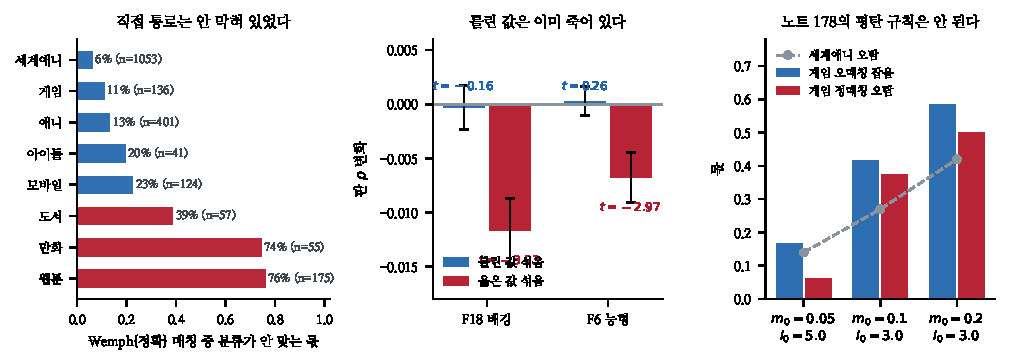
\includegraphics[width=\textwidth]{figs/dead.pdf}
\caption{왼쪽 --- 직접 통로는 안 막혀 있었다. 가운데 --- 틀린 값을 섞어도
아무 일도 안 난다. 오른쪽 --- 노트 178의 평탄 규칙은 안 된다.}
\end{figure*}

\section{하루 만에 내 제안을 반증했다}

\begin{table}[t]
\centering\tsize
\caption{노트 178의 평탄 규칙. 게임 포함 매칭 28건에 손 라벨.}
\begin{tabular}{llrrr}
\toprule
$m_0$ & $l_0$ & 오매칭 잡음 & 정매칭 오탐 & 세계애니 오탐 \\
\midrule
0.05 & 5.0 & 2/12 & 1/16 & 14\% \\
0.10 & 3.0 & 5/12 & 6/16 & 27\% \\
0.20 & 3.0 & 7/12 & \textbf{8/16} & \textbf{42\%} \\
\bottomrule
\end{tabular}
\end{table}

\claimx{\textbf{옳은 것을 틀린 것만큼 잡는다.} 어느 문턱에서도 잡음과
오탐이 거의 같고, 낱개 자질의 AUC 는 변동 0.630 · 봉우리 0.635 · 기울기
0.609 다.}{까닭이 보인다 --- 세계애니의 포함 매칭도 평평하다(변동
0.304). 게임의 오매칭(0.292)과 구별이 안 된다. \textbf{평평함은 일반
명사의 표지가 아니라 \emph{옛 문서}의 표지다.}}

\claimx{\textbf{여섯 번째다.} 노트 157$\to$158 · 158$\to$159 ·
163$\to$169 · 165$\to$166 · 173$\to$174, 그리고 178$\to$179.}{노트 174가
``한 사례에서 세운 규약은 대개 너무 넓다''로 적은 자리다. 이번 것은
사례가 \textbf{하나}였다 --- 게임의 목록을 눈으로 본 것.}

\section{되는 것은 분류였다}

\begin{table}[t]
\centering\tsize
\caption{분류 규칙. 게임 포함 매칭 28건 손 라벨.}
\begin{tabular}{lrr}
\toprule
& 잡음 & 오탐 \\
\midrule
\textbf{분류 안 맞으면 버림} & \textbf{7/12} & \textbf{0/16} \\
\bottomrule
\end{tabular}
\end{table}

\claimx{\textbf{정밀도가 완전하다}(오탐 0/16). ``Backrooms (film)''은 영화
분류만, ``Drone racing''은 분류가 아예 없고, ``물''은 무기 화합물 ·
산화물이다. ``Blue Archive''는 비디오 게임 분류를 갖는다.}{재현율은
7/12 다 --- ``Train simulator''가 ``Video game genres'' 분류를 갖고 있어
통과한다. \textbf{장르 문서는 못 거른다.}}

\claimx{\textbf{판이 아니라 의미로 정한 규칙이다.} 분류가 안 맞으면 그
문서는 그 IP 가 아니다 --- 판을 보고 문턱을 고르는 노트 178의 자리와
근거의 성질이 다르다.}{낱말 목록은 손으로 만든 것이라 완전하지 않다.
모바일에서 보드게임 원작(``Terra Mystica'')을 오탐하던 것을 보고
``board game''을 넣었다. \textbf{목록을 고칠 때 판을 안 봤다.}}

\section{직접 통로가 열려 있었다}

\begin{table}[t]
\centering\tsize
\caption{\emph{정확} 매칭(score 1.0) 중 분류가 안 맞는 몫.}
\begin{tabular}{lrr}
\toprule
& n & 안 맞음 \\
\midrule
\textbf{웹툰} & 175 & \textbf{76.0\%} \\
\textbf{만화} & 55 & \textbf{74.5\%} \\
도서 & 57 & 38.6\% \\
모바일 & 124 & 22.6\% \\
아이돌 & 41 & 19.5\% \\
애니 & 401 & 13.2\% \\
게임 & 136 & 11.0\% \\
세계애니 & 1053 & 6.2\% \\
\bottomrule
\end{tabular}
\end{table}

\claimx{\textbf{노트 150은 검색 통로만 막았다.} 겹침 검사는
\texttt{list=search} 결과에만 붙어 있고 \texttt{direct()} 는 제목이 문서
이름과 정확히 같으면 무조건 붙인다.}{웹툰 ``해귀''$\to$임진왜란,
``아르마딜로''$\to$빈치류, ``하우스키퍼''$\to$동음이의어 문서. 도서
``아몬드''$\to$벚나무속, ``희망''$\to$감정, ``급류''$\to$육수학. 만화
``Centuria''$\to$로마 군단, ``NeuN''$\to$항체.}

\claimx{\textbf{score 1.0 이라 노트 178의 문턱으로는 안 보인다.} 노트
178이 ``정확만($\ge$1.0)''을 제일 깨끗한 칸으로 놓고 표를 그렸는데
\textbf{그 칸이 제일 더러운 칸이었다} --- 웹툰에서 76\%다.}{제목이 짧고
흔한 낱말일수록 위험하다. \textbf{한국어 웹툰 제목이 그렇게 생겼다.}}

\section{그런데 버려도 판이 안 움직인다}

\begin{table}[t]
\centering\tsize
\caption{분류가 안 맞는 행을 결측으로 돌리면.}
\begin{tabular}{lrrl}
\toprule
& 차 & sd & \\
\midrule
F18 배깅 & $-$.0001 & .0030 & $t{=}-0.02$ \\
F6 능형 & $+$.0031 & .0024 & $t{=}1.31$ \\
\bottomrule
\end{tabular}
\end{table}

\claimx{\textbf{내 예측이 틀렸다.} $+$0.003$\sim$$+$0.012 를 적었는데
$-$0.0001 이다. 웹툰 정확 매칭의 76\%를 버렸는데 웹툰 $\rho$ 가 0.0021
움직인다.}{두 읽기가 있었다 --- 틀린 값을 빼서 오르거나, 마스크를 잃어서
내리거나(노트 176). \textbf{둘 다 아니었다.}}

\section{섞어 보니 까닭이 나온다}

\begin{table}[t]
\centering\tsize
\caption{값을 레코드 사이에서 섞는다. 마스크는 그대로. 짝 부트스트랩 400회.}
\begin{tabular}{lrrl}
\toprule
& 차 & sd & \\
\midrule
\multicolumn{4}{l}{\emph{F18 배깅}} \\
\textbf{틀린 값 섞음} & \textbf{$-$.0003} & .0020 & $t{=}-0.16$ \\
옳은 값 섞음 & $-$.0117 & .0030 & \textbf{$t{=}-3.93$} \\
\multicolumn{4}{l}{\emph{F6 능형}} \\
\textbf{틀린 값 섞음} & \textbf{$+$.0003} & .0013 & $t{=}0.26$ \\
옳은 값 섞음 & $-$.0068 & .0023 & \textbf{$t{=}-2.97$} \\
\bottomrule
\end{tabular}
\end{table}

\claimx{\textbf{틀린 값은 이미 죽어 있었다.} 섞어도 두 형태 다 0 에서 안
갈리고, 옳은 값을 섞으면 둘 다 갈린다. \textbf{버리는 것과 놔두는 것이
같은 까닭이 이것이다} --- 이미 아무 일도 안 하고 있었다.}{노트 176의
마스크 섞기와 정확히 같은 얼개다. 거기서는 참 마스크가 $+$0.0063
($t{=}2.3$)로 갈렸고 여기서는 틀린 값이 안 갈린다. \textbf{같은 자로 두
가지를 쟀다.}}

\claimx{\textbf{그러니 판 $\rho$ 로는 자료가 맞는지 알 수 없다.} 3,653행
중 406행(11.1\%)이 엉뚱한 문서인데 판정치는 그것을 못 본다 --- 넣어도
빼도 섞어도 같다.}{노트 176이 ``판이 내려가는 것이 나쁜 모형을 뜻하지
않는다''를, 노트 178이 ``판이 올라가는 것도 좋은 자료를 뜻하지 않는다''를
세웠다. \textbf{여기는 셋째다 --- 판이 안 움직이는 것도 자료가 맞다는
뜻이 아니다.}}

\section{그래서 채택한다}

\claimx{\textbf{판을 안 올리는데 채택한다.} 노트 178에서는 판을 올리는
것($+$0.0050)을 안 채택했고 여기서는 안 올리는 것($-$0.0001)을
채택한다. \textbf{두 결정의 기준이 같다} --- 판이 아니라 ``그 문서가 그
IP 인가''다.}{채택의 값은 판이 아니라 \emph{배포}에서 나온다. 새 웹툰
``해귀''의 사전 관심도로 임진왜란 문서 조회수를 쓰는 모형은, 판이
어떻든 기획자에게 내놓을 수 없다.}

\begin{table}[t]
\centering\tsize
\caption{남은 것.}
\begin{tabular}{ll}
\toprule
\textbf{웹툰 · 만화} & 76\% · 74.5\% 를 버리면 위키 축이 남나 \\
장르 문서 & ``Video game genres'' 를 못 거른다 \\
낱말 목록 & 손으로 만든 것 --- 도메인마다 검증 안 했다 \\
\bottomrule
\end{tabular}
\end{table}

첫 줄이 곧바로 잴 수 있다. 웹툰은 유보 711건에 위키 덮음이 11.9\%였는데
분류 검사 뒤 \textbf{7.0\%}가 된다. 만화도 18.4\%에서 16.7\%다.
\textbf{그 정도 덮음으로 축 넷을 세울 값이 있는지가 다음 자리다} ---
노트 149가 위키를 들인 까닭이 ``만화 · 세계애니의 검색 덮음 0\%를
채운다''였는데, 만화에서 채운 것의 74.5\%가 엉뚱한 문서였다.

\end{document}
